\documentclass{article}
\usepackage{amsmath}
\usepackage{amssymb}
\usepackage{bm}
\let\biconditional\leftrightarrow
\usepackage{hyperref}
\usepackage{graphicx}

\newcommand{\lolly}{-\!\!\ast~}

% Tabbing \tab	
\usepackage{tabto}
\NumTabs{4}

% For specifying colours.
\usepackage{color}
\definecolor{darkGrey}{rgb}{0.35,0.35,0.35}
\definecolor{medGrey}{rgb}{0.5,0.5,0.5}
\definecolor{medGreen}{rgb}{0.0,0.4,0.15}
\definecolor{medOrange}{rgb}{0.7,0.3,0.0}
\definecolor{lightGrey}{rgb}{0.98,0.98,0.98}
\definecolor{lightViolet}{rgb}{0.7,0.35,0.7}
\definecolor{darkPurp}{rgb}{0.4,0.1,0.4}
\definecolor{black}{rgb}{0.1,0.1,0.1}
\definecolor{white}{rgb}{1.0,1.0,1.0}

% Monospaced font.
\usepackage{courier}

% Used for code highlighting.
\usepackage{listings}
\newcommand\codestyle{
   \lstset{
      aboveskip=10pt,
      belowskip=5pt,
      backgroundcolor=\color{white},
      basicstyle=\ttfamily\footnotesize\color{black},
      frame=single,
      showstringspaces=false
   }
}


\lstnewenvironment{code}[1][]
{
\codestyle
\lstset{#1}
}
{}

\usepackage{graphicx}

\setlength{\parindent}{0pt}

\begin{document}

\paragraph{}
This document describes architectural patterns we may wish to describe in Wyvern using a declarative logic/language extension. In diagrams a box represents a module. A directed arrow with an open head connects module $A$ to module $B$ if $A$ has a reference to module $B$. A collection of modules may be enclosed within a coloured box. This represents the boundaries of the system.

\section{Layers}

\paragraph{}
A layered architecture is a hierarchy of modules. In each layer in the hierarchy the modules talk only to modules in the layers above or below (usually). An example is the TCP/IP protocol stack. Another is shown below where a client can make database queries to a server. The server's architecture is divided into four layers $L_1, ..., L_4$. The first three layers abstract the data stored in the database at increasingly high levels. $L_4$ handles networking and provides an interface to the client.

\paragraph{}
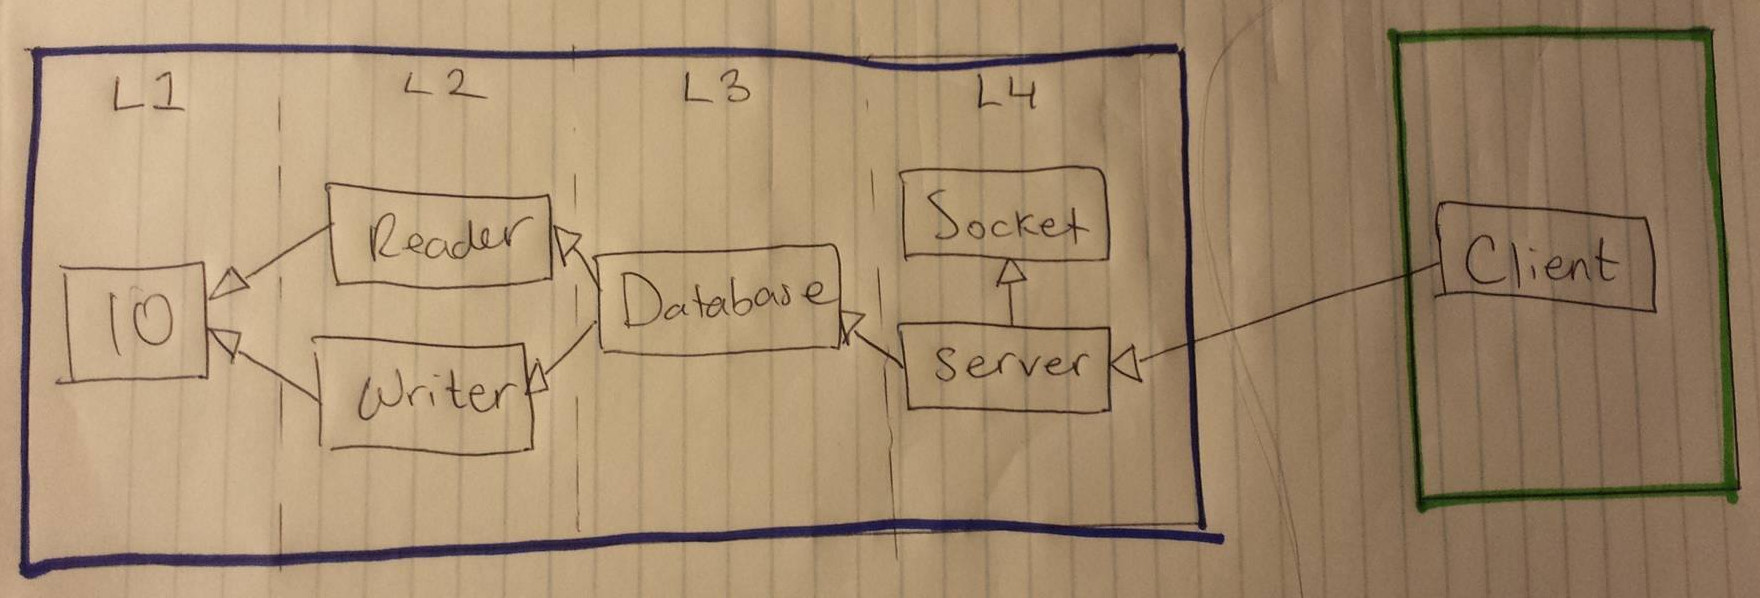
\includegraphics[width=\textwidth]{layers.jpeg}

\paragraph{}
$L_4$ should not directly use modules on $L_1$ to perform data reads/writes. It should only do so through $L_3$, the database layer. The client, which is external to the layered system, interacts only through the topmost layer $L_4$. These highlight some properties of layered designs:
\begin{itemize}
	\item Placing internal restrictions on how the layers interact. An implementation satisfying a layered architecture should only message-pass through the interfaces of the layers.
	\item Placing restrictions on how external programs interact with the layered system as a whole.
\end{itemize}

\section{Pipeline}

\paragraph{}
A pipeline architecture performs a sequence of transformations on input data. Its output is transformed data, which has been passed through a series of independent components called filters. The output of each filter is passed into the input of the next filter. An example of a pipeline is an interpreter, where source code undergoes multiple transformations before its output is interpreted. A diagram of the Wyvern interpreter pipeline is given below.

\paragraph{}
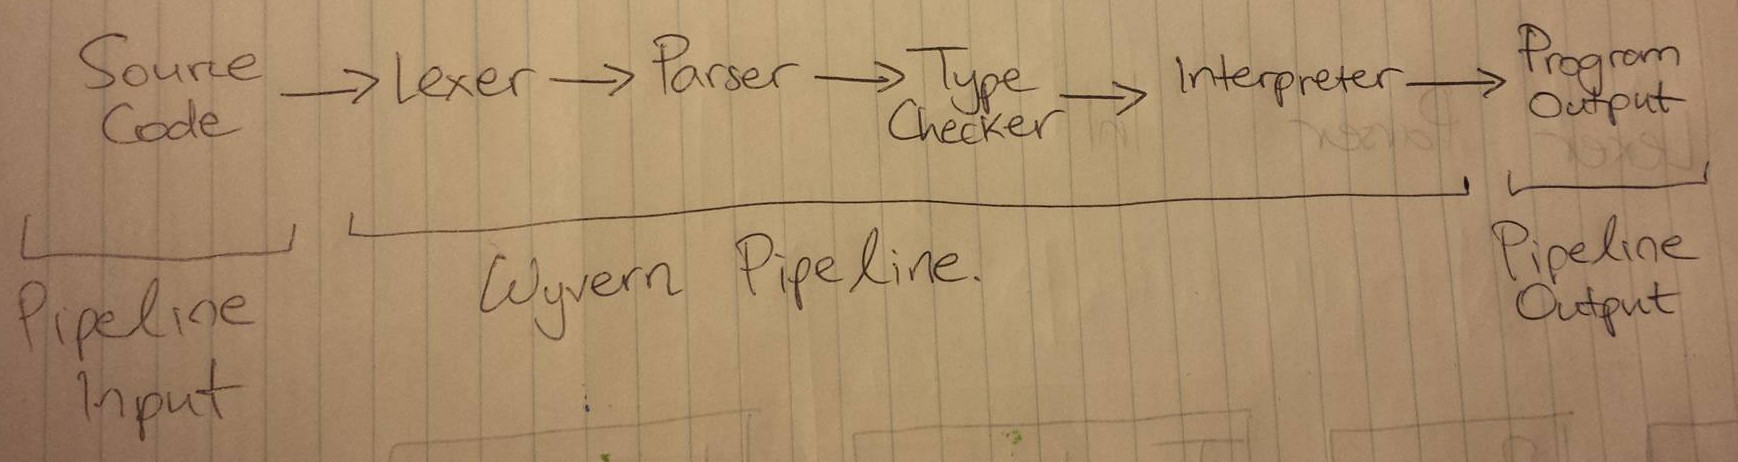
\includegraphics[width=\textwidth]{pipeline.jpeg}

\paragraph{}
Important properties of a pipeline design:
\begin{itemize}
	\item Preserving the integrity of data as they leave one filter and enter the next. The system may wish to do something with the intermediate representation (e.g. save it to a file) but this should not change the intermediate representation.
	\item Describe how the filters fit together. Architectural constraints should be general enough that each filter can vary independently of the others.
	\item Because pipelines are sequential, linear-temporal predicates may be useful.
\end{itemize}

\section{Event Sequencing}

\paragraph{}
Resources such as files and sockets can be in an open or closed state. More complex state machines, such as user interfaces, can be in a large number of complicated states. In all of these we usually want invariants to say that by the end of computation they must be in a certain state. Such architectures are concerned with constraining the shape of programs which use them: a program using a socket can do whatever it wants, but every $open$ must be followed by a $close$ in order for the socket to function correctly.

\paragraph{}
Examples:
\begin{itemize}
	\item Every file or socket which is opened must be closed.
	\item Queries to a database must be sanitised before being processed by a server (to protect agains e.g. SQL injections). This is most important when the sanitation and processing logic are in separate modules.
	\item Data must be passed through an appropriate encryption module before it is sent through a socket.
	\item Because this deals with a sequence of events, temporal predicates may be useful.
\end{itemize}

\section{Dynamic Plugins}

\paragraph{}
A system like that given in the ECOOP '16 paper may provide some means of software extension by third-party plugins. A big concern is how we can trust third-party plugins to make sure they don't do things such as abuse the UserInfo module. A simplified diagram of the ECOOP '16 paper is given below. More generally we want to impose constraints about how programs external to the architecture may use it. This is related to specifying a clean interface for the system as a whole.

\paragraph{}
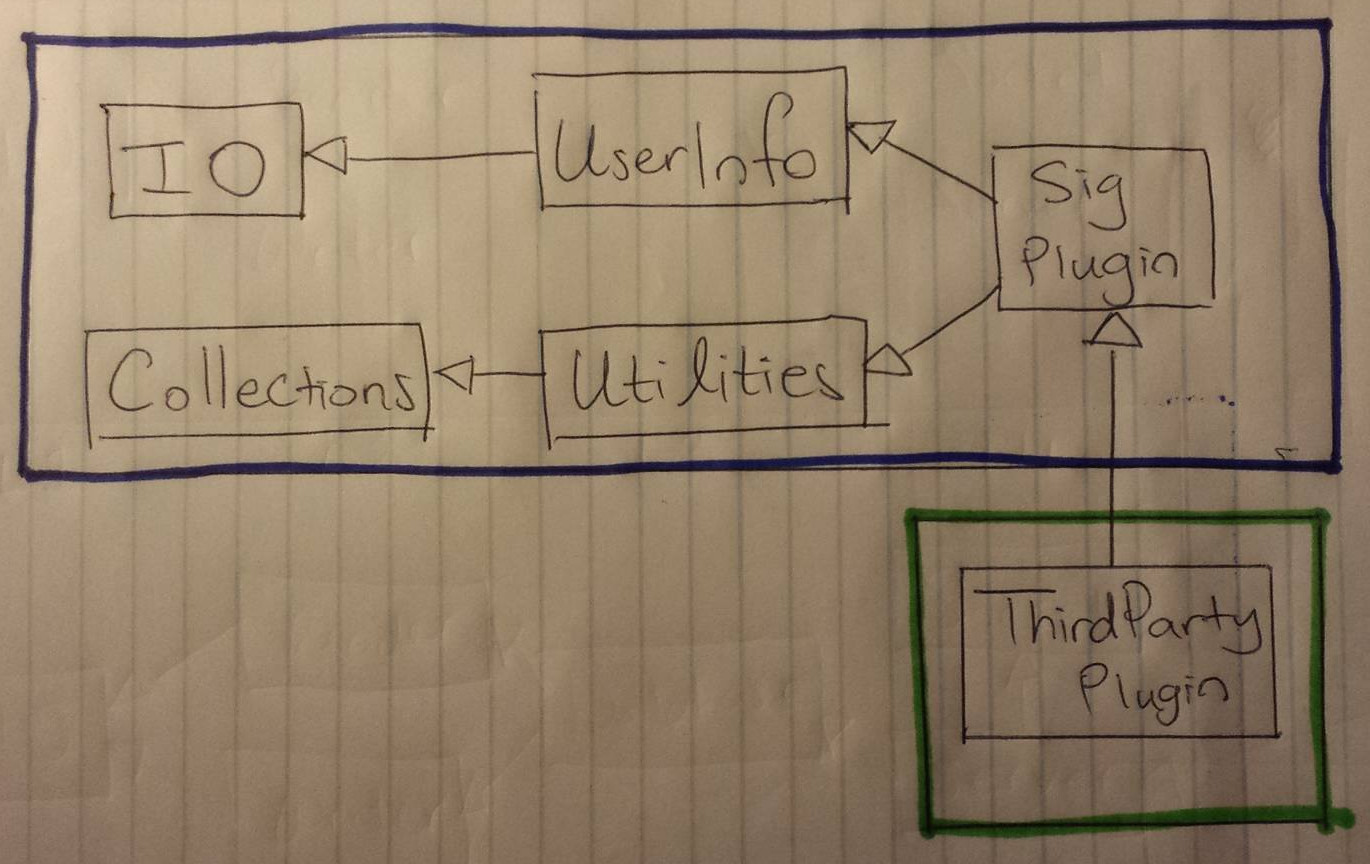
\includegraphics[width=\textwidth]{plugins.jpeg}

\paragraph{}
An architecture should:
\begin{itemize}
	\item Be able to specify when a plugin is violating use of the API. If a third-party plugin is deemed malicious it could be passed a benign, dummied-out reference to the UserInfo module so it cannot do any harm.
	\item Runtime granting and revocation of module capabilities.
\end{itemize}

\section{Service Mediators}

\paragraph{}
A service mediator $M$ provides some service to an existing module $A$ by interacting with another module $B$. $M$ abstracts the information flow between $A$ and $B$. Examples include service locators and resource schedulers. Below is a web browser that uses $ResourceLocater$ as a service loactor for URIs.

\paragraph{}
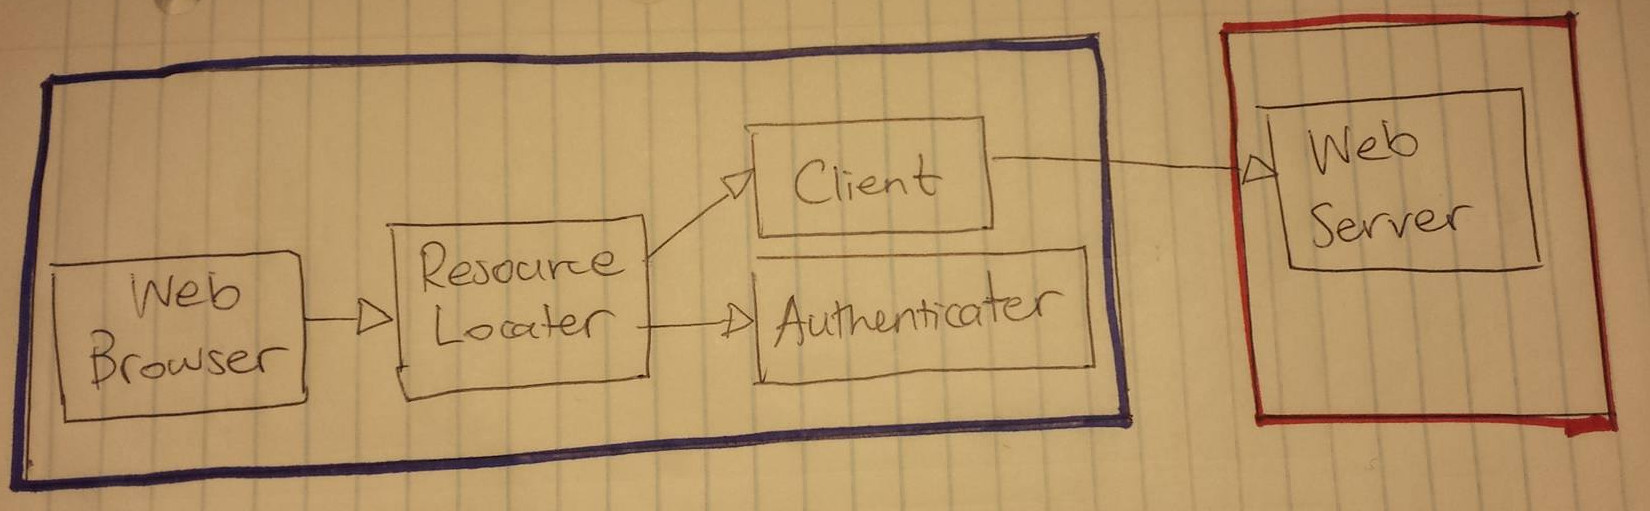
\includegraphics[width=\textwidth]{service-mediator.jpeg}

\paragraph{}
Because $M$ is supposed to encapsulate the flow of information from $A$ to $B$, a valid implementation should not talk to anyone $A$ doesn't know about. In the below example, $A$ talks to $B$ via $M$. $M$ is leaking $A$'s information to a malicious third-party module that $A$ does not know about, when $M$ is only supposed to be encapsulating a conversation between $A$ and $B$.

\paragraph{}
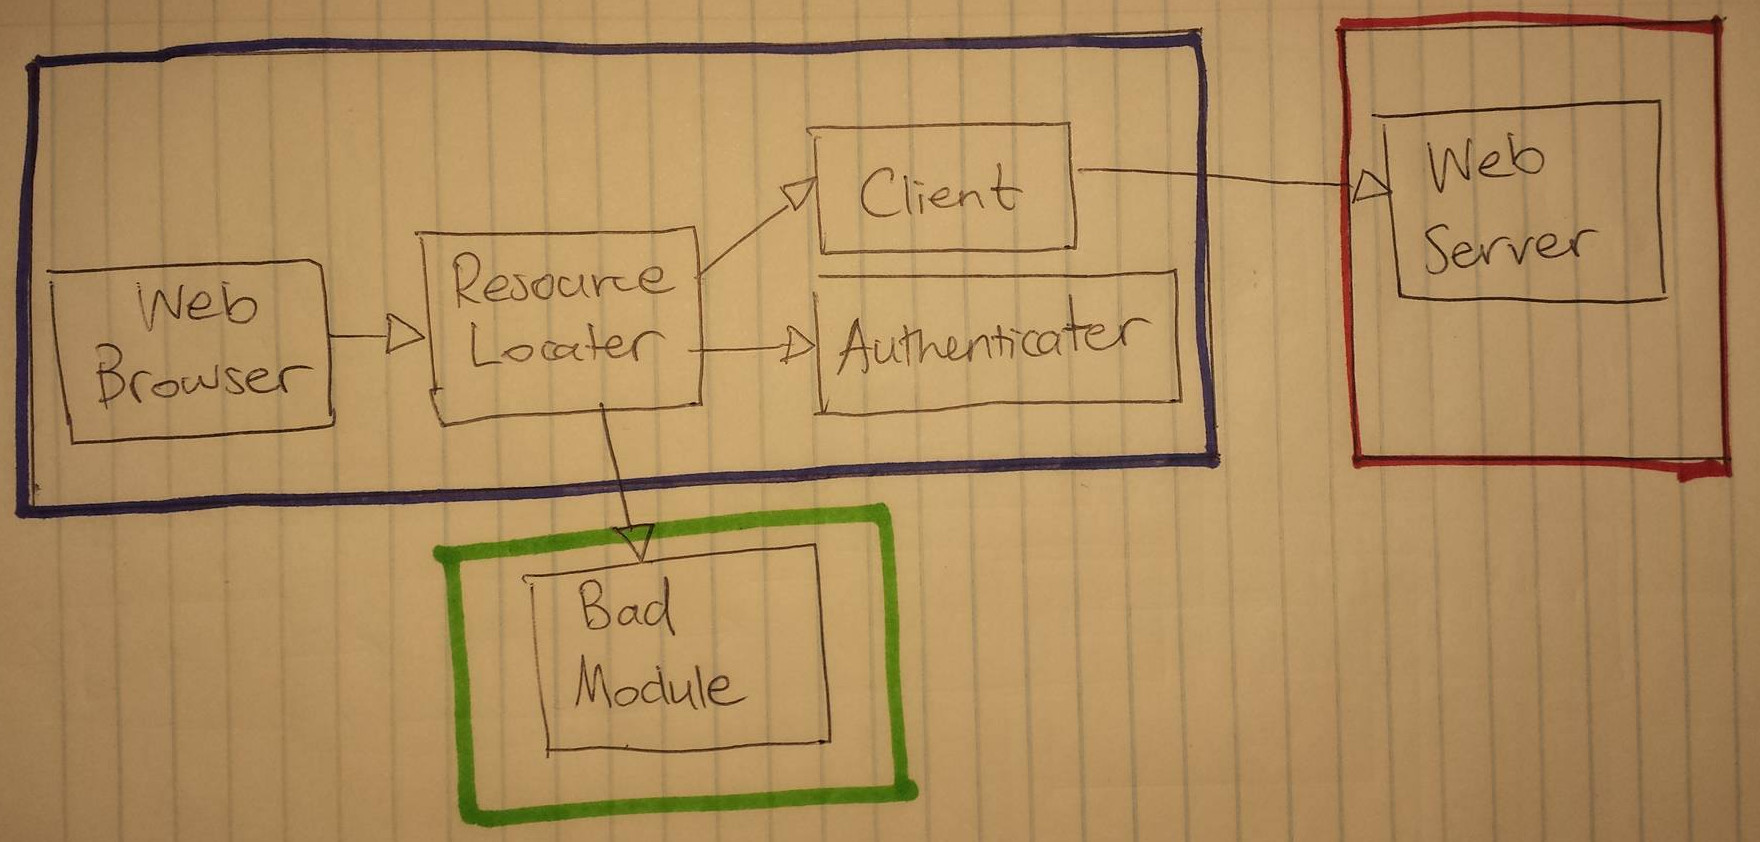
\includegraphics[width=\textwidth]{service-mediator-bad.jpeg}

\paragraph{}
A harder problem would be figuring out that $M$ is returning accurate results. Since $A$ delegates to $M$ in order to perform service location, a malicious implementation of $M$ might intentionally give the wrong answers to $A$ (for example, by not talking to $B$ at all and merely returning an empty file!).

\begin{itemize}
	\item Prevent a mediator $M$ talking to parties unknown to $A$.
	\item Ensuring $M$ actually performs service location correctly with the intended recipient of $A$'s message.
\end{itemize}

\section{Conversation Mediators}

A mediator $M$ may also be an intermediary between a whole bunch of modules on an equal level. In the diagram below $M$ is mediating a conversation between $A$, $B$, and $C$. Though these modules are collectively in one big conversation, the flow of information between modules may be quite strict. We want $M$ to preserve those information flows. The information flows might be synchronous or asynchronous. In the below diagram, $I_{A \rightarrow B}$ and $I_{A \rightarrow C}$ are two information flows from $A$ to $B$ and $A$ to $C$ respectively. A rogue mediator might send each information to the wrong recipient. 

\paragraph{}
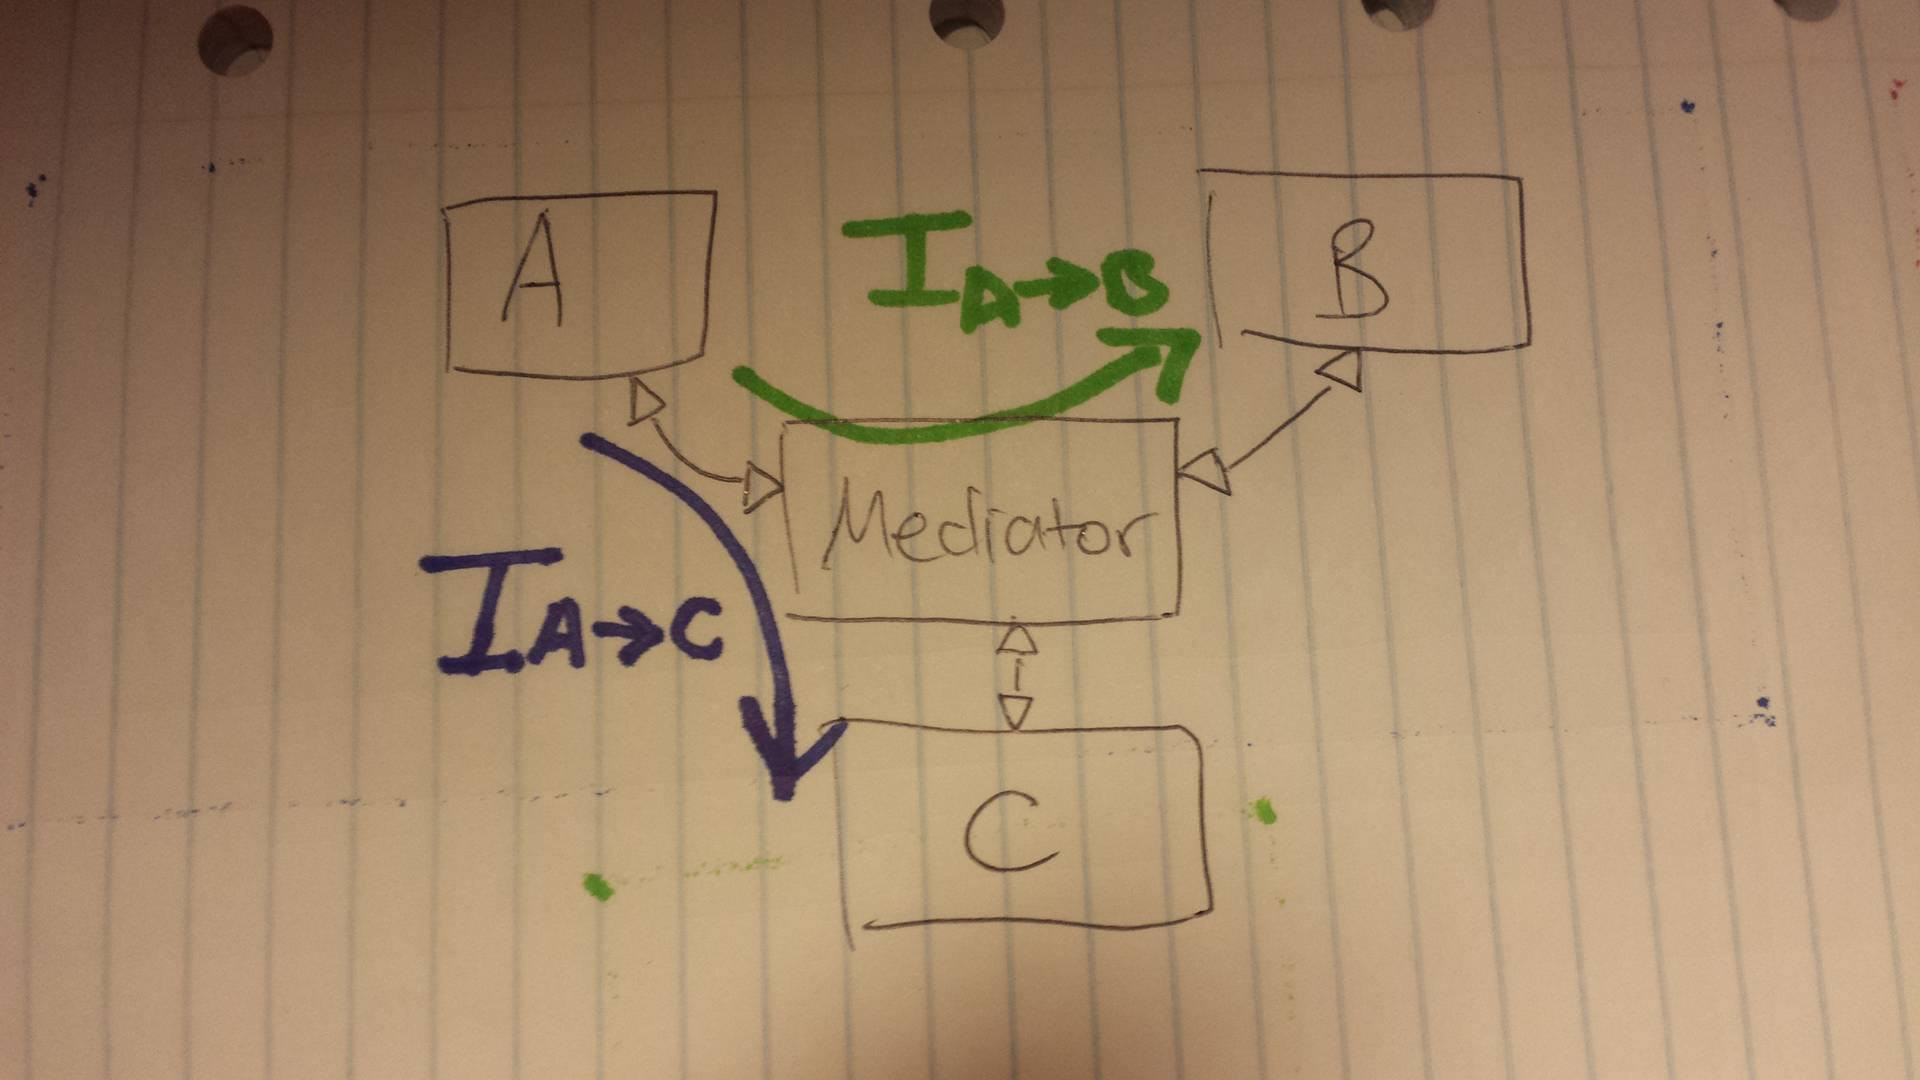
\includegraphics[width=\textwidth]{conversation-mediator.jpeg}

\paragraph{}
An architecture should be able to:
\begin{itemize}
	\item Explain which modules are talking to who in a conversation so the mediator doesn't leak information.
	\item Specify how they're talking to each other (e.g. $A$ might talk to $B$ through some method of $M$ called $AtoB$).
\end{itemize}

\section{Event Systems}

\paragraph{}
Some architectures run on an event-based system. An example is a user interface, where a click event or button event prompts an action listener and/or event handler to respond to the event. Applications which have to model continuous time (e.g. videogames and simulations) may have an event queue where a central control module pops events off the queue and notifies the parties interested in the event. A complicated system may several modules running independently which communicate via asynchronous event system.

\paragraph{}
The system below is a simplified version of one described in \textit{Software Architecture and Practice} by \textit{Bass et al}. It is a flight simulator for the United States military. Two kinds of agents participate in the simulator: $pilots$ and $instructors$ (who can also control aspects of the simulator). A $synchroniser$ module pops events off a queue and sends news about those events to the relevant subsystem responsible for that part of the simulation.

\paragraph{}
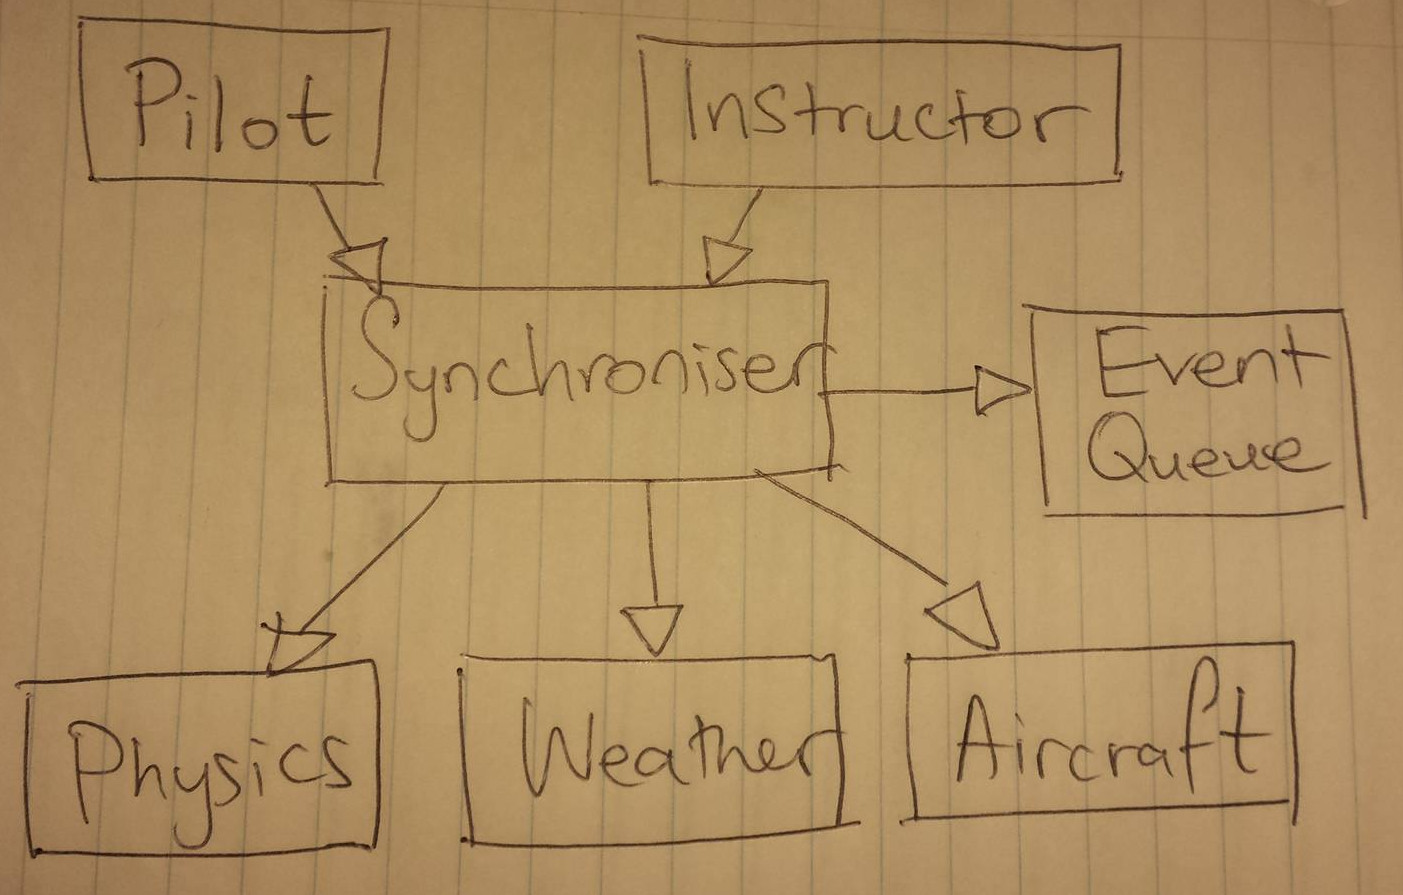
\includegraphics[width=\textwidth]{aircraft-sim.jpeg}

Concerns include:
\begin{itemize}
	\item Declare events that can be sent and received.
	\item Which modules are sending events? In our example, only $pilot$ and $instrutor$ can send events.
	\item Of those modules which can send events, what events are they allowed to send? In this situation only $instructors$ may send events which change the parameters of the simulation.
	\item Which modules should be notified that an event has fired? In this case, the $physics$, $weather$, and $aircraft$ modules.
	\item Is the event handler notifying the right people? If an event fires to say that a pilot took damage, that information should be passed to the $aircraft$ module and not the $weather$ module.
\end{itemize}

\end{document}

